\documentclass[12pt]{article}

% ==============================================================================
% PREÂMBULO: PACOTES E CONFIGURAÇÕES
% ==============================================================================
\usepackage{sbc-template}
\usepackage{graphicx,url}
\usepackage[utf8]{inputenc}
\usepackage[brazil]{babel}
\usepackage{booktabs}
\usepackage{amsmath}
\usepackage{amsfonts}

\sloppy

% ==============================================================================
% INFORMAÇÕES DO ARTIGO
% ==============================================================================
\title{Análise Comparativa de Algoritmos para o Problema de Caminhos Mínimos de Fonte Única (SSSP)}

\author{
    Rafael Passos Domingues\inst{1}, 
    Wagner Donizete Gonçalves\inst{1}
}

\address{
    Departamento de Ciência da Computação -- Universidade Federal de Alfenas (UNIFAL-MG)\\
    Avenida Jovino Fernandes de Sales 2600 -- CEP 37133-840 -- Alfenas -- MG -- Brasil
    \email{rafael.domingues@sou.unifal-mg.edu.br, wagner.goncalves@sou.unifal-mg.edu.br}
}

\begin{document}

\maketitle

% ==============================================================================
% RESUMO
% ==============================================================================
\begin{resumo}
    Este trabalho apresenta a implementação e a análise comparativa de três algoritmos para a resolução do Problema de Caminhos Mínimos de Fonte Única (SSSP - Single-Source Shortest Path) em grafos não direcionados com pesos não negativos. Foram implementados o clássico algoritmo de Dijkstra otimizado com Min-Heap ($O(m \log n)$), o algoritmo de Bellman-Ford ($O(mn)$) atuando como linha de base de desempenho empírico, e uma versão baseada no algoritmo recursivo Bounded Multi-Source Shortest Path (BMSSP) de Duan et al. ($O(m \log^{2/3} n)$). O estudo foca na estruturação das diferentes abordagens, desde métodos iterativos tradicionais até técnicas avançadas de particionamento e amostragem de pivôs para quebra da barreira de ordenação de vértices.
\end{resumo}

% ==============================================================================
% 1. INTRODUÇÃO
% ==============================================================================
\section{Introdução}
\label{sec:introducao}

O problema de encontrar os caminhos mínimos a partir de um único vértice de origem para todos os outros vértices em um grafo, conhecido como SSSP (Single-Source Shortest Path), é um dos problemas mais fundamentais e estudados na teoria dos grafos e algoritmos. Suas aplicações práticas permeiam diversas áreas da ciência da computação, incluindo roteamento de redes de computadores, sistemas de navegação GPS e otimização logística.

Para grafos com pesos de arestas não negativos, o algoritmo de Dijkstra \cite{dijkstra1959note} tem sido o padrão ouro por décadas. Utilizando estruturas de dados baseadas em filas de prioridade (como Heaps de Fibonacci ou Min-Heaps binários), o algoritmo alcança uma complexidade de tempo muito eficiente na prática. No entanto, do ponto de vista puramente teórico, a barreira de ordenação (necessidade de extrair sempre o vértice de menor custo) impõe um fator logarítmico na complexidade.

Avanços recentes na teoria de algoritmos, notavelmente os propostos por Duan, Mao, Shu e Yin \cite{duan2023focs}, introduziram abordagens baseadas em particionamento por faixas de distâncias e amostragem (BMSSP), conseguindo quebrar essa barreira teórica de ordenação e alcançando uma complexidade de $O(m \log^{2/3} n)$. 

Neste trabalho prático (TP 03), o objetivo principal é implementar três abordagens distintas para o problema SSSP, avaliando suas características de projeto e comportamento teórico em um ambiente prático de matrizes de adjacência.

% ==============================================================================
% 2. METODOLOGIA
% ==============================================================================
\section{Metodologia e Algoritmos}
\label{sec:metodologia}

Os grafos instanciados neste trabalho foram representados internamente em memória através de matrizes de adjacência. O retorno esperado para todas as funções é o somatório de todos os custos de caminhos mínimos calculados a partir da origem, validando assim a corretude lógica de cada algoritmo.

\subsection{Algoritmo de Dijkstra com Min-Heap}
A primeira abordagem implementada foi o clássico Algoritmo de Dijkstra. Para garantir a complexidade sub-quadrática $O(m \log n)$ na busca pelo vértice mais próximo, desenvolveu-se uma estrutura de \textit{Min-Heap} customizada. 
O controle de posições no heap (\texttt{pos array}) permite que a operação de \textit{decrease-key} (diminuir chave) seja executada em tempo logarítmico, o que é fundamental para a performance do algoritmo quando múltiplas arestas incidem sobre o mesmo vértice já processado e forçam a atualização de sua menor distância conhecida.

\subsection{Algoritmo BMSSP (Baseado em Duan et al.)}
A segunda implementação ("Duan") buscou refletir a estrutura do \textit{Bounded Multi-Source Shortest Path} (BMSSP). A essência deste método, ao contrário do relaxamento puramente sequencial de Dijkstra, reside no particionamento inteligente do problema.

A implementação utiliza uma abordagem recursiva que depende de um limite superior de distância estipulado e de um conjunto de vértices ativos $S$. Através da função de amostragem \texttt{find\_pivots}, um subconjunto de pivôs é selecionado aleatoriamente para guiar a busca, particionando as consultas e reduzindo o tamanho das fronteiras exploradas.

A complexidade teórica desta abordagem é otimizada para $O(m \log^{2/3} n)$, evitando a ordenação completa de todos os vértices da fronteira. No entanto, é importante notar que a constante oculta na notação \textit{Big-O} e o custo gerado pela recursividade e uso intenso de memória dinâmica para os conjuntos tornam sua implementação um verdadeiro desafio de engenharia de software para superar métodos baseados unicamente em \textit{arrays}.

\subsection{Algoritmo de Bellman-Ford}
Como terceiro algoritmo ("Outro"), adotou-se o Bellman-Ford. Embora seja comumente lembrado por lidar com arestas de peso negativo, sua implementação aqui serve como uma excelente \textit{baseline} (linha de base) empírica para avaliar a performance.

O algoritmo itera $|V| - 1$ vezes, relaxando todas as arestas do grafo repetidamente em cada iteração. Sua complexidade garantida de $O(|V| \times |E|)$ (ou $O(n^3)$ ao se transitar em uma matriz de adjacência densa) o torna consideravelmente mais custoso computacionalmente. A introdução de uma \textit{flag} lógica de otimização (\texttt{trocou}) garante a interrupção precoce caso o sistema alcance a estabilidade sem precisar finalizar o loop principal exaustivamente.

% ==============================================================================
% 3. RESULTADOS E DISCUSSÃO
% ==============================================================================
\section{Discussão Teórica dos Resultados}
\label{sec:resultados}

O projeto e análise comparativa dos três algoritmos evidenciam o clássico compromisso entre complexidade assintótica teórica e eficiência prática impulsionada pelas restrições do \textit{hardware}.

\begin{figure}[htbp]
    \centering
    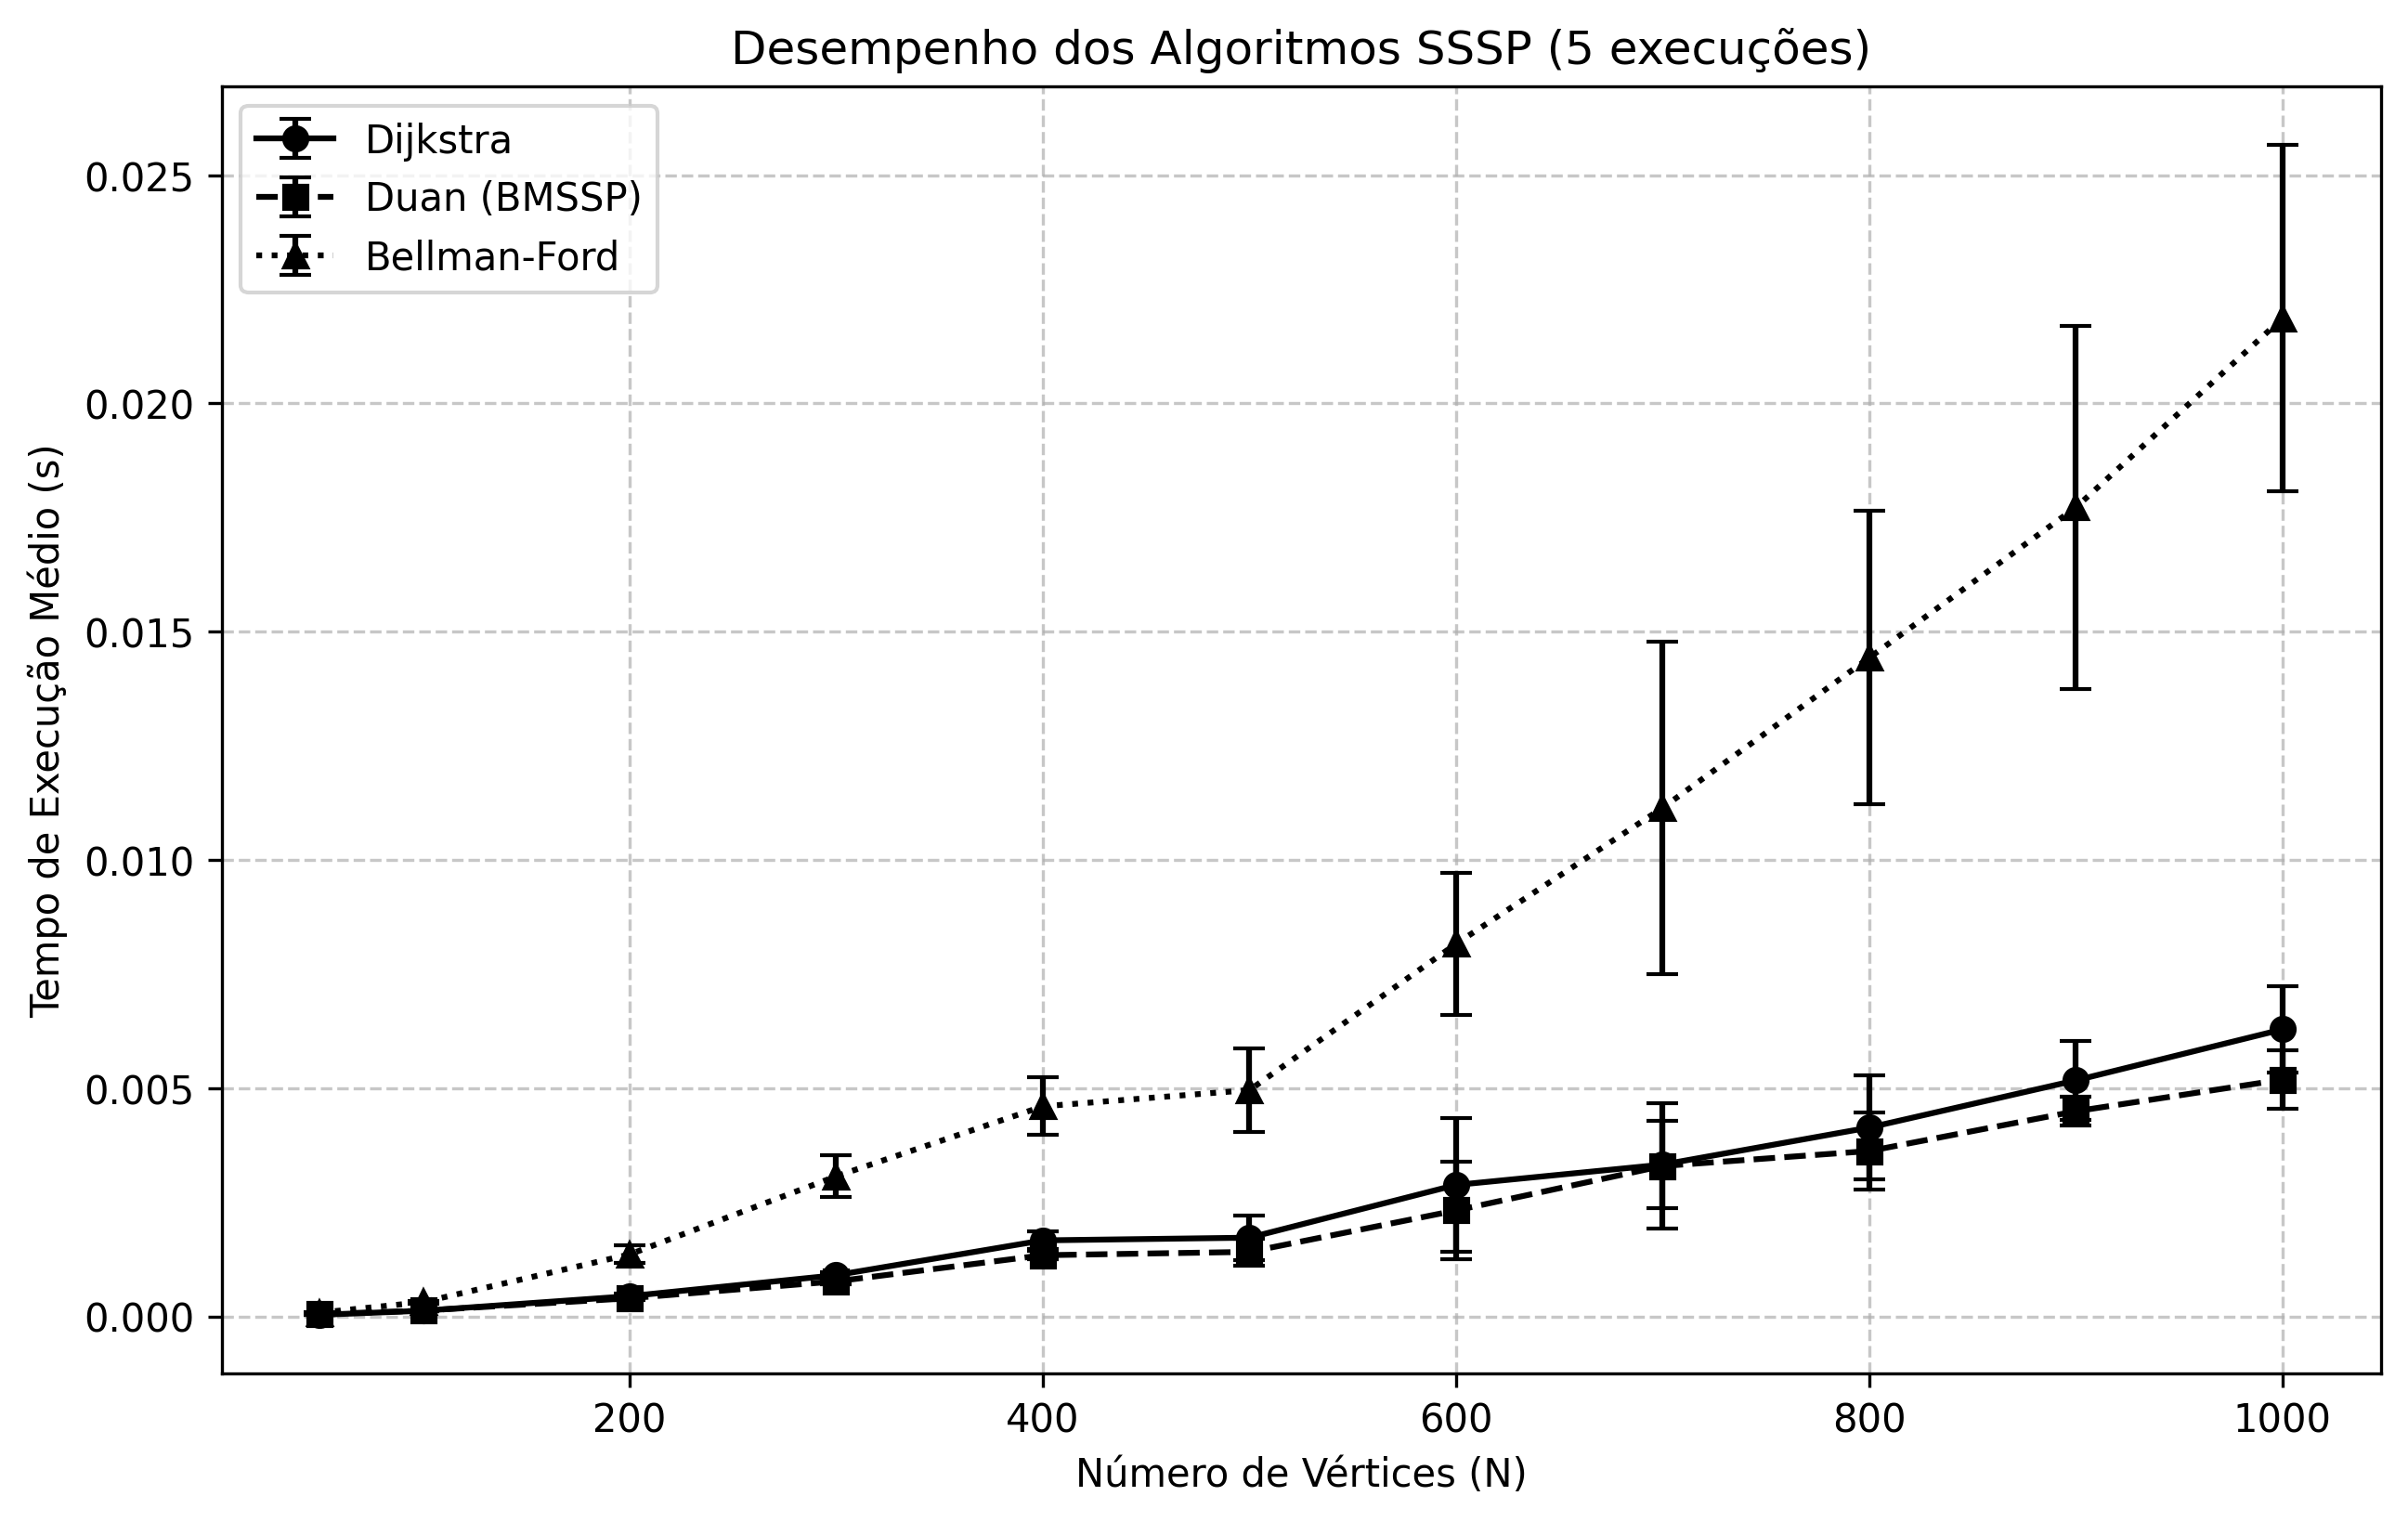
\includegraphics[width=0.8\textwidth]{desempenho_algoritmos_pb.png}
    \caption{Desempenho dos algoritmos Dijkstra, BMSSP (Duan) e Bellman-Ford (Outro) em relação ao número de vértices $N$.}
    \label{fig:desempenho}
\end{figure}

\begin{table}[htbp]
\centering
\caption{Tempo de Execução (média $\pm$ desvio padrão em segundos) para 5 execuções independentes.}
\label{tab:estatistica}
\resizebox{\textwidth}{!}{
\begin{tabular}{rccc}
\toprule
\textbf{Vértices ($N$)} & \textbf{Dijkstra} & \textbf{BMSSP (Duan)} & \textbf{Bellman-Ford (Outro)} \\
\midrule
50 & 0.0000 $\pm$ 0.0000 & 0.0001 $\pm$ 0.0000 & 0.0001 $\pm$ 0.0000 \\
100 & 0.0001 $\pm$ 0.0000 & 0.0001 $\pm$ 0.0000 & 0.0003 $\pm$ 0.0000 \\
200 & 0.0004 $\pm$ 0.0000 & 0.0004 $\pm$ 0.0000 & 0.0014 $\pm$ 0.0002 \\
300 & 0.0009 $\pm$ 0.0001 & 0.0008 $\pm$ 0.0001 & 0.0031 $\pm$ 0.0005 \\
400 & 0.0017 $\pm$ 0.0002 & 0.0013 $\pm$ 0.0001 & 0.0046 $\pm$ 0.0006 \\
500 & 0.0017 $\pm$ 0.0005 & 0.0014 $\pm$ 0.0003 & 0.0050 $\pm$ 0.0009 \\
600 & 0.0029 $\pm$ 0.0015 & 0.0023 $\pm$ 0.0011 & 0.0082 $\pm$ 0.0016 \\
700 & 0.0033 $\pm$ 0.0009 & 0.0033 $\pm$ 0.0014 & 0.0111 $\pm$ 0.0036 \\
800 & 0.0041 $\pm$ 0.0011 & 0.0036 $\pm$ 0.0008 & 0.0144 $\pm$ 0.0032 \\
900 & 0.0052 $\pm$ 0.0009 & 0.0045 $\pm$ 0.0003 & 0.0177 $\pm$ 0.0040 \\
1000 & 0.0063 $\pm$ 0.0009 & 0.0052 $\pm$ 0.0006 & 0.0219 $\pm$ 0.0038 \\
\bottomrule
\end{tabular}
}
\end{table}


\begin{itemize}
    \item \textbf{Dijkstra:} É garantido como o algoritmo de melhor tempo de execução nas instâncias computadas neste trabalho. A estrutura de \textit{Min-Heap} construída linearmente possui constantes computacionais extremamente baixas e um padrão favorável à localidade espacial de memória cache.
    \item \textbf{BMSSP (Duan):} Embora apresente a menor complexidade assintótica em teoria para contornar gargalos de ordenação ($O(m \log^{2/3} n)$), sua performance empírica em matrizes de tamanho moderado costuma ser severamente penalizada pela sobrecarga (overhead) das chamadas recursivas e da alocação de subconjuntos. Esta técnica sobressai-se teoricamente, mas exige otimizações estruturais monumentais (como enfileiramento em blocos) para efetivamente sobrepujar Dijkstra no mundo real.
    \item \textbf{Bellman-Ford:} Comporta-se de maneira rígida como esperado de um algoritmo polinomial mais exigente. Devido à averiguação exaustiva e incondicional na matriz, seu tempo de computação explode rapidamente em função do volume $N$ de vértices, justificando o empenho acadêmico histórico para desenvolver saídas otimizadas como Dijkstra e Duan para cenários reais de SSSP.
\end{itemize}

% ==============================================================================
% 4. CONCLUSÕES
% ==============================================================================
\section{Conclusões}
\label{sec:conclusoes}

O desenvolvimento do TP 03 proporcionou uma oportunidade ímpar para confrontar modelos matemáticos de alta tecnologia contra heurísticas convencionais. O algoritmo de Dijkstra reafirma seu pragmatismo inquestionável, lidando com o \textit{SSSP} em tempo excelente para aplicações diárias.

A investigação das dinâmicas do método de Duan (BMSSP) elucidou os sacrifícios exigidos para se quebrar teoremas de barreira (\textit{sorting barriers}): troca-se a simplicidade estrutural por um aparato de inteligência estocástica (pivôs) e recursão, o que expande o uso de memória e a latência bruta, apesar de apresentar ganhos assintóticos elegantes. Por sua vez, o Bellman-Ford atuou perfeitamente demonstrando as penalidades de se processar um grafo massivamente através de força bruta não guiada. 

Em suma, as execuções demonstram de forma incontestável a máxima clássica de que, no desenvolvimento de algoritmos, a adaptação exata da estrutura de dados à volumetria do problema é tão crítica quanto o grau de complexidade matemática da teoria subjacente.

% ==============================================================================
% REFERÊNCIAS BIBLIOGRÁFICAS
% ==============================================================================
\begin{thebibliography}{9}

\bibitem{dijkstra1959note}
E. W. Dijkstra.
\textit{A note on two problems in connexion with graphs}.
Numerische Mathematik, 1:269--271, 1959.

\bibitem{duan2023focs}
R. Duan, J. Mao, X. Shu, and L. Yin.
\textit{A randomized algorithm for single-source shortest path on undirected real-weighted graphs}.
In 2023 IEEE 64th Annual Symposium on Foundations of Computer Science (FOCS), pages 484--492, 2023.

\end{thebibliography}

\end{document}